\documentclass[letterpaper]{article} % DO NOT CHANGE THIS
\usepackage[submission]{aaai2027}  % DO NOT CHANGE THIS
\usepackage[hyphens]{url}  % DO NOT CHANGE THIS
\usepackage{graphicx} % DO NOT CHANGE THIS
\urlstyle{rm} % DO NOT CHANGE THIS
\def\UrlFont{\rm}  % DO NOT CHANGE THIS
\usepackage{natbib}  % DO NOT CHANGE THIS AND DO NOT ADD ANY OPTIONS TO IT
\usepackage{caption} % DO NOT CHANGE THIS AND DO NOT ADD ANY OPTIONS TO IT
\frenchspacing  % DO NOT CHANGE THIS

% AAAI-27 Deployable AI Workshop submission (long track, 7 pages of main text;
% references and appendices excluded). Adapted from ../naacl2027/main.tex with
% a deployment-first framing; the evidence is unchanged. Tables in tables/ are
% generated by make_tables.py; do not hand-edit them. Table~\ref{tab:failures}
% is hand-authored here because it carries no new number: every figure in it
% is restated from the body.
\usepackage{booktabs}
\usepackage{array}
\usepackage{tikz}
\usetikzlibrary{positioning,fit,backgrounds,shadows,arrows.meta}
\usepackage{listings}
\lstdefinestyle{promptstyle}{
  basicstyle=\scriptsize\ttfamily,
  breaklines=true,
  breakatwhitespace=false,
  breakindent=0pt,
  postbreak=\mbox{$\hookrightarrow$\space},
  columns=fullflexible,
  keepspaces=true,
  showstringspaces=false,
  frame=none,
  numbers=none,
  xleftmargin=0pt,
  aboveskip=4pt, belowskip=4pt,
  literate={—}{{---}}1 {–}{{--}}1 {≤}{{$\leq$}}1 {→}{{$\rightarrow$}}1
  {“}{{``}}1 {”}{{''}}1 {‘}{{`}}1 {’}{{'}}1 {…}{{\ldots}}1
  {≥}{{$\geq$}}1 {×}{{$\times$}}1 {½}{{$\frac{1}{2}$}}1
}

\pdfinfo{
  /TemplateVersion (2027.1)
}

\setcounter{secnumdepth}{2} % numbered sections, allowed by the template

% Marks figures that come from deployment logs and engineering notes rather
% than from a recorded evaluation artifact (see the opening of Section 6).
\newcommand{\elog}{\textsuperscript{$\ddagger$}}

\title{From PDF to Structured Data: Deploying an LLM Pipeline to Make\\
US Early Learning Standards Machine-Readable}
\author{Anonymous Submission}
\affiliations{}

\begin{document}

\maketitle

\begin{abstract}
  US states publish early learning standards for preschool-age children mostly
  as PDFs, each in its own design, so this body of public policy does not exist
  as structured data. We report on deploying an LLM pipeline that converts these
  documents into one queryable schema, in which every extracted standard becomes
  a record that downstream applications and human reviewers depend on.
  Deployment imposed requirements that extraction benchmarks do not: new
  documents without new code, keys that are reproducible across runs of a
  sampling model, nothing structurally impossible persisted, bounded cost, and
  failures that are visible. The detector meets the first by classifying each
  element by its nesting position against a depth map inferred per document in a
  cheap first pass. On annotated subsets of six states, detector recall is 1.000
  at every level in the recorded run (at least 0.978 in repeats) and an audit of
  297 detections finds one hallucination; ablating the depth map degrades
  exactly the positional levels, and a rule-based extractor matches the method
  only at the top level. Inference for one state's complete standards
  (41--52 pages) costs about \$4. Most of the remaining requirements were met by moving
  every rule with a single correct output out of the model and into code, and by
  validating at the persistence boundary. Four of the six deployment failures we
  report surfaced only on whole documents in production, including a run that
  reported success while losing most of its document.
\end{abstract}

% =====================================================================
\section{Introduction}
\label{sec:introduction}

Early learning standards are the developmental expectations that shape
curriculum, assessment, and teacher preparation for children before
kindergarten entry. More than fifty US jurisdictions issue them for
preschool-age children~\citep{ncecqa_elgs} and each designs its own document.
Unlike K--12 academic standards, which have machine-readable exchange
formats~\citep{sutton2008achievement,1edtech2017case}, early learning standards
exist almost entirely as PDFs: multi-column tables, age-banded grids and prose
whose typography is not commonly shared. Curriculum-planning tools, alignment
studies and cross-state comparisons all need them as structured data, and
today that data is produced by hand, if at all.

Turning these documents into data is a deployment problem before it is an
extraction problem. The pipeline's output is not a benchmark answer but a
database row whose identifier,
\texttt{\{country\}-\{state\}-\{year\}-}\allowbreak\texttt{\{indicator\_code\}},
is a primary key
read by a state standards explorer. An
indicator means something only through its ancestry (which domain, strand and
sub-strand it sits under, and at what age band), so a misplaced level or a key
that changes between runs is a data-integrity failure, not a scoring error.
And the surface cues that reveal ancestry are exactly what varies: Arizona
writes \texttt{Strand 1: Language and Literacy}; Kentucky writes
\texttt{Benchmark 1.1}; Nevada prints a code namespace that skips a level;
Colorado has no sub-strand tier at all. A rule tuned to one document's
vocabulary fails on the next, and no annotated corpus exists to learn the
mapping from.

We describe a system that recovers this structure with in-context LLM calls
and runs as a serverless pipeline on AWS. Its detector classifies elements by
nesting position, not label: a first, cheap pass infers a per-document depth
map, and every element is then classified against that map.
\texttt{Benchmark 1.1} need not be recognized as a ``sub-strand'', only as
sitting one level below \texttt{Language and Early Literacy Standard 1}. A
parser resolves the detected elements into one canonical schema with
deterministic identifiers, a validator guards the database, and a human can
review every stored record in an editorial interface. The system runs end to
end in production infrastructure and is in pre-launch use as the data layer
behind both applications.

Our central observation is that the system became deployable less by making
the model more accurate than by deciding what the model is allowed to decide.
It makes the judgments no rule can make across documents; everything with a
single correct output (an abbreviation, a uniqueness tie-break, a structural
invariant, whether a run is healthy) is taken away from it.

\paragraph{Contributions.} (1)~Deployment requirements for LLM extraction
whose output is stored as records that applications depend on, and a system that meets them with no
per-state code path: two-pass detection by per-document depth map, and a
parser that resolves six independently designed documents into one schema
with reproducible keys (\S\ref{sec:requirements}--\ref{sec:method}).
(2)~An evaluation on six states covering quality, an ablation, a rule-based
baseline, run-to-run stability, and whole-document scale and cost
(\S\ref{sec:eval}). (3)~A record of six deployment failures, where each
surfaced and what now guards it, distilled into practices for deploying LLMs
whose outputs are stored as data (\S\ref{sec:lessons}).

% =====================================================================
\section{Related Work}
\label{sec:related}

\paragraph{Document hierarchy.} Layout analysis and OCR-free transcription
recover text and page
objects~\citep{lopez2009grobid,zhong2019publaynet,xu2020layoutlm,huang2022layoutlmv3,kim2022donut,blecher2023nougat},
and hierarchical document parsing reconstructs logical trees by learning from
annotated renderings of a genre with consistent
typography~\citep{rausch2021docparser,ma2023hrdoc,wang2024detect,xing2024dochienet,wang2025unihdsa}.
Our setting has neither. Training-free neighbors segment law books from
table-of-contents cues~\citep{wehnert2025hips} or prompt for a pseudo table of
contents for retrieval~\citep{jeong2025docsray}; our depth map is the
table-of-contents subtask of \citet{wang2024detect}, inferred zero-shot and
used as the authority for every classification.

\paragraph{LLM extraction without labels.} Generative extraction is
competitive where labeled data is
scarce~\citep{agrawal2022large,wadhwa2023revisiting,xu2024large}, though
fine-tuning wins where labels exist~\citep{liu2022fewshot}.
GoLLIE~\citep{sainz2024gollie} trains models to follow annotation guidelines;
our prompts state document-agnostic structural guidelines to a frozen model.
We validate JSON and repair it deterministically rather than constraining
decoding~\citep{willard2023efficient}, chunk by domain given long-context
degradation~\citep{liu2024lost}, and audit for
hallucination~\citep{ji2023survey}. Human effort goes to blanket verification
rather than to annotation or confidence-guided
review~\citep{monarch2021human,settles2009active,li2023coannotating}.

\paragraph{Deploying learned systems.} Production ML accumulates failure modes
that sit outside the model~\citep{sculley2015hidden,paleyes2022challenges},
and readiness rubrics ask for validation of data at system boundaries and for
parity between the code that is tested and the code that
serves~\citep{breck2017mltestscore,breck2019datavalidation}. LLMs add output
that varies across identical requests~\citep{ouyang2023nondeterminism}. Our
validator applies boundary validation to model output, as
\citet{aggarwal2025fiscal} do for fiscal tables, and our lessons report
concrete instances of these risks in an LLM pipeline whose outputs are stored
as data. Unlike those case studies, the pipeline has no training step: every
component is a prompt, a frozen model or deterministic code, so a model update
is a prompt edit, and we key every recorded result to a hash of the source that
holds the prompts.

\paragraph{Machine-readable standards.} ASN~\citep{sutton2008achievement} and
CASE~\citep{1edtech2017case} model and exchange K--12 standards, and alignment
work assumes a normalized set already
exists~\citep{porter2002measuring,polikoff2011howwell,devaul2011computer,xu2025automated}.
For early childhood, it does not: the one federal framework binds only Head
Start~\citep{ohs2015elof}. This paper automates that missing input.

% =====================================================================
\section{Deployment Setting and Requirements}
\label{sec:requirements}\label{sec:data}\label{sec:corpus}\label{sec:schema}

\paragraph{Canonical schema.} The target schema has four levels,
\emph{domain}, \emph{strand}, \emph{sub-strand} and \emph{indicator}, of which
the middle two are optional, because a four-level schema is not a four-level
document: Colorado publishes no sub-strand tier, and forcing one would require
inventing structure. Each level has a code, a name and an optional
description; the indicator also carries an age band, a source page and the
verbatim source text. The unit of storage is a leaf with its full lineage,
keyed by the identifier above, whose indicator code is fully qualified and
carries any side-by-side disambiguator itself: an age column appends its month
range (Texas \texttt{I.A.2.36-48} vs.\ \texttt{I.A.2.48-60}, and likewise
California's age columns), and a proficiency column its label (California
\texttt{ELD.1.0.VOCA.1.1.DISC}). Every level also carries human-verification
state (Appendix~\ref{sec:appendix-schema}).

\paragraph{Corpus and tiers.} We use documents from six states: four for
development (AZ, CA, CO, TX) and two for validation (NV, KY). No code path
names any state, but validation-state failures prompted several general fixes
during development, so the set is \emph{not} a clean held-out test
(\S\ref{sec:limitations}). Each document exists at up to three tiers. The \emph{full} tier
is the published PDF. The \emph{trimmed} tier removes front matter, essays,
and appendices but \textbf{retains every standard}, so it reduces cost but not
coverage. The \emph{subset} tier is one to two domains per state, 70 pages and
262 standards in total, annotated for grading (\S\ref{sec:eval});
\textbf{all headline quality numbers are at this tier}. Both cuts were made by
hand, which favors the system; Appendix~\ref{sec:appendix-corpus} lists every
source document and the retained pages.

\paragraph{Requirements.} Five requirements came from deployment rather than
from the extraction task, and organize the rest of the paper:
\textbf{R1}~a new state's document is processed without new code;
\textbf{R2}~a standard's key is reproducible from the document, not from the
order or the run in which the pipeline processed it;
\textbf{R3}~no structurally impossible record is persisted, and every stored
record is cheap for a human to check against its source;
\textbf{R4}~a whole document runs within serverless time limits and model
quotas at a cost of a few dollars;
\textbf{R5}~a run that loses data says so.
R1--R4 are met by the design of \S\ref{sec:method}; R5 is only partly met, and
\S\ref{sec:lessons} says why.

% =====================================================================
\section{System}
\label{sec:method}

% Deployed architecture, full width, read left to right. Hand-authored TikZ:
% it depicts the deployed topology, not measured data. Replaces the review
% build's use of ../figures/fig_architecture.pdf
% (paper/analysis/make_architecture_figure.py), whose labels shrank to 1.9pt at
% text width. Keep in sync with documentation/ARCHITECTURE.md: ten Lambda
% handlers (the gray boxes), Pass 1 runs in the detection prepare handler, and
% every stage boundary is an S3 write and read.
%
% Geometry is explicit so the six cards fit \textwidth (16cm) at 8pt text:
% four single-handler cards 1.95cm wide, two batched cards 2.8cm, 0.38cm gaps.
\begin{figure*}[t]
\centering
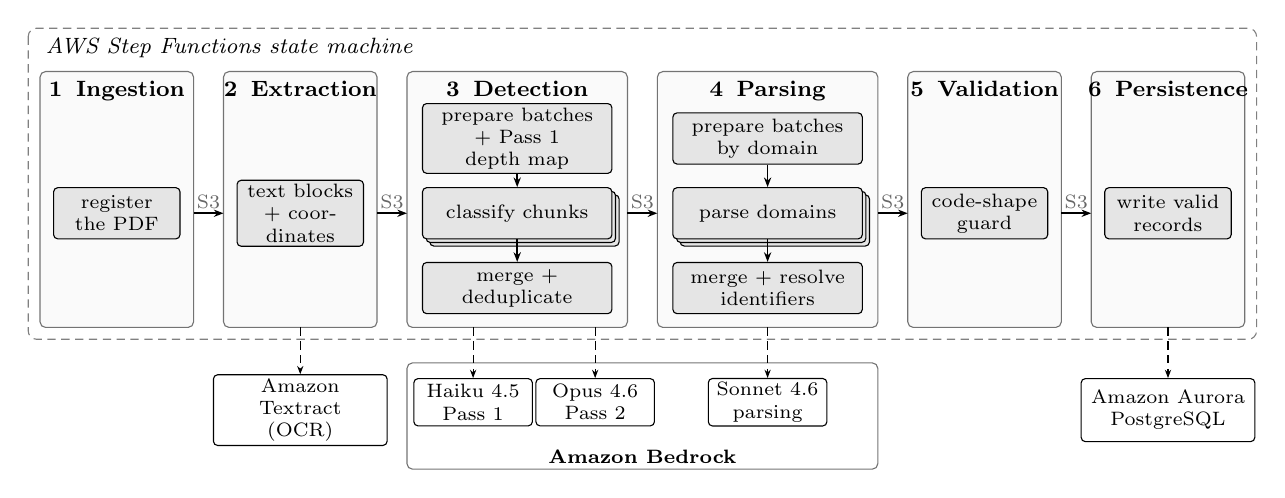
\begin{tikzpicture}[
  x=1cm, y=1cm,
  card/.style={draw=black!55, rounded corners=2pt, fill=black!2},
  ctitle/.style={font=\footnotesize\bfseries, anchor=north, inner sep=0pt},
  fn/.style={draw, rounded corners=1.5pt, fill=black!10, font=\scriptsize,
    align=center, text width=#1, minimum height=6.5mm, inner sep=1.5pt},
  fn/.default=15mm,
  mapfn/.style={fn=#1, double copy shadow={shadow xshift=1.3pt,
    shadow yshift=-1.3pt, fill=black!10, draw}},
  mapfn/.default=15mm,
  svc/.style={draw, rounded corners=1.5pt, fill=white, font=\scriptsize,
    align=center, text width=#1, minimum height=8mm, inner sep=1.5pt},
  svc/.default=17mm,
  flow/.style={-{Stealth[length=3.5pt]}, semithick},
  call/.style={-{Stealth[length=3pt]}, densely dashed},
  s3/.style={font=\scriptsize, text=black!60, above, inner sep=1.5pt},
]
% Card spans (left, right) and centers.
\def\cardA{0}     \def\cardAr{1.95}   \def\cA{0.975}
\def\cardB{2.33}  \def\cardBr{4.28}   \def\cB{3.305}
\def\cardC{4.66}  \def\cardCr{7.46}   \def\cC{6.06}
\def\cardD{7.84}  \def\cardDr{10.64}  \def\cD{9.24}
\def\cardE{11.02} \def\cardEr{12.97}  \def\cE{11.995}
\def\cardF{13.35} \def\cardFr{15.30}  \def\cF{14.325}
\def\ctop{0}      \def\cbot{-3.25}    \def\cmid{-1.8}

% Orchestration frame.
\draw[black!50, densely dashed, rounded corners=3pt]
  (-0.15, 0.55) rectangle (15.45, -3.4);
\node[font=\footnotesize\itshape, anchor=west] at (-0.05, 0.3)
  {AWS Step Functions state machine};

% Stage cards.
\foreach \l/\r/\c/\t in {\cardA/\cardAr/\cA/1\enspace Ingestion,
                         \cardB/\cardBr/\cB/2\enspace Extraction,
                         \cardC/\cardCr/\cC/3\enspace Detection,
                         \cardD/\cardDr/\cD/4\enspace Parsing,
                         \cardE/\cardEr/\cE/5\enspace Validation,
                         \cardF/\cardFr/\cF/6\enspace Persistence} {
  \draw[card] (\l, \ctop) rectangle (\r, \cbot);
  \node[ctitle] at (\c, \ctop - 0.12) {\t};
}

% Lambda handlers: one per single-handler card, three per batched card.
\node[fn] (ing) at (\cA, \cmid) {register\\ the PDF};
\node[fn] (ext) at (\cB, \cmid) {text blocks\\ + coordinates};
\node[fn=23mm] (dprep) at (\cC, -0.85) {prepare batches\\ + Pass 1 depth map};
\node[mapfn=23mm] (dmap) at (\cC, \cmid) {classify chunks};
\node[fn=23mm] (dmerge) at (\cC, -2.75) {merge + deduplicate};
\node[fn=23mm] (pprep) at (\cD, -0.85) {prepare batches\\ by domain};
\node[mapfn=23mm] (pmap) at (\cD, \cmid) {parse domains};
\node[fn=23mm] (pmerge) at (\cD, -2.75) {merge + resolve\\ identifiers};
\node[fn] (val) at (\cE, \cmid) {code-shape\\ guard};
\node[fn] (per) at (\cF, \cmid) {write valid\\ records};

\draw[flow] (dprep) -- (dmap);
\draw[flow] (dmap) -- (dmerge);
\draw[flow] (pprep) -- (pmap);
\draw[flow] (pmap) -- (pmerge);

% Stage to stage: every hand-off is a JSON write and read through S3.
\foreach \a/\b in {\cardAr/\cardB, \cardBr/\cardC, \cardCr/\cardD,
                   \cardDr/\cardE, \cardEr/\cardF} {
  \draw[flow] (\a, \cmid) -- node[s3] {S3} (\b, \cmid);
}

% External services. The Bedrock label sits at the bottom of its box so the
% call arrows from above never cross it.
\node[svc=21mm] (ocr) at (\cB, -4.3) {Amazon Textract\\ (OCR)};
\draw[black!55, rounded corners=2pt] (\cardC, -3.7) rectangle (\cardDr, -5.05);
\node[font=\scriptsize\bfseries, anchor=south, inner sep=2pt]
  at ({(\cardC+\cardDr)/2}, -5.05) {Amazon Bedrock};
\node[svc=14mm, minimum height=6mm] (haiku) at (5.5, -4.2) {Haiku 4.5\\ Pass 1};
\node[svc=14mm, minimum height=6mm] (opus) at (7.05, -4.2) {Opus 4.6\\ Pass 2};
\node[svc=14mm, minimum height=6mm] (sonnet) at (\cD, -4.2) {Sonnet 4.6\\ parsing};
\node[svc=21mm] (db) at (\cF, -4.3) {Amazon Aurora\\ PostgreSQL};

\draw[call] (\cB, \cbot) -- (ocr);
\draw[call] (5.5, \cbot) -- (haiku);
\draw[call] (7.05, \cbot) -- (opus);
\draw[call] (\cD, \cbot) -- (sonnet);
\draw[call] (\cF, \cbot) -- (db);
\end{tikzpicture}
\caption{Deployed architecture, read left to right. Each gray box is one of the
ten AWS Lambda handlers; stacked boxes fan out through a Step Functions
\texttt{Map} state with at most three concurrent workers. Every hand-off between
stages is a JSON write and read through Amazon S3. Dashed arrows are calls to
external services; only records that pass validation are persisted.}
\label{fig:architecture}
\end{figure*}


The pipeline has six stages (Figure~\ref{fig:architecture}).
\emph{Ingestion} registers a PDF; \emph{extraction} recovers text blocks with
page coordinates from Textract OCR repaired against the PDF's own text layer;
\emph{detection} emits a flat list of typed elements; \emph{parsing} resolves
them into the schema; \emph{validation} checks structural invariants;
\emph{persistence} writes surviving records to PostgreSQL. Stages are Lambda
functions that exchange JSON through S3, so any stage can be replayed in
isolation from the previous stage's output. Detection and parsing are batched
through a prepare~$\rightarrow$~Step Functions
\texttt{Map}~$\rightarrow$~merge pattern (at most three concurrent workers) so
that a long document does not exhaust a function timeout (R4).

\paragraph{Two stages, two questions.} Detection answers \emph{what is on the
page}: a local judgment. Parsing answers \emph{what it is a child of}: a global
one, since a parent may be printed pages earlier. Each stage sees the context
it needs (parsing reasons over a whole domain at once), is graded against its
own golden, and runs on the cheapest adequate model (R4): the depth-map pass on
Claude Haiku~4.5, detection on Claude Opus~4.6, parsing on Claude Sonnet~4.6,
all at temperature zero.

\subsection{Detection}
\label{sec:method-detection}

\paragraph{Pass 1: depth map.} One call infers how many nesting levels the
document uses and how each is rendered (Appendix~\ref{sec:prompt-depthmap}).
Every element's level is later assigned against this map, so \emph{a level
missing from Pass~1's input is missing from the whole run}. The pass sees a
6{,}000-token sample, and sampling matters: headings are rare and prose
abundant, so every-$n$th sampling drops the lines that establish the top of
the hierarchy (\S\ref{sec:lessons}). We instead bucket blocks by their
normalized left edge, since indentation tracks nesting and a rare x-position is
a rare depth; each bucket receives a floor of twelve blocks spread across the
document, rarest buckets first, and the remaining budget goes to the bulk.

\paragraph{Pass 2: classification.} The document is chunked into
${\sim}$2{,}000 token windows with 500 tokens of overlap, and each chunk is
classified with the depth map as context. The central instruction is
positional: classify an element by where it sits in the map, not by its label
word (Appendix~\ref{rule:positional}). Supporting rules are equally general
(R1): in a \texttt{<Label> <id>: <Title>} heading, for \emph{any} label word,
the label and id are the code; a printed code is authoritative and may appear
inline, in a caption, or as the shared prefix of the element's descendants'
codes. If the document does not print a code, one is derived from the title by
a fixed abbreviation procedure (Appendix~\ref{rule:code-resolution}).

\subsection{Parsing and identifiers}
\label{sec:method-parsing}

% Table 1 belongs to Section 5, but a full-width float can appear at the
% earliest on the page after the one that defines it, so it is input here.
% AUTO-GENERATED by paper/dai2027/make_tables.py -- do not hand-edit.
% Source: paper/results/task1_20260826/summary.json, task2_20260826/summary.json, the signed FP audits, corpus_tiers.json
% Regenerate with: python paper/dai2027/make_tables.py
\begin{table*}[t]
  \centering
  \small
  \begin{tabular}{lrrrrrrr}
    \toprule
    & & & \multicolumn{2}{c}{\textbf{Detection}} & \multicolumn{3}{c}{\textbf{Parsing}} \\
    \cmidrule(lr){4-5} \cmidrule(lr){6-8}
    \textbf{State} & \textbf{pp} & \textbf{Std.} & \textbf{Ver.\ prec.} & \textbf{Code acc.} & \textbf{Coverage} & \textbf{Field acc.} & \textbf{Fully corr.} \\
    \midrule
    AZ & 15 & 45 & 1.000 & 4/4 & 18/18 & 0.997 & 17/18 \\
    CA & 13 & 94 & 1.000 & 25/25 & 21/21 & 1.000 & 21/21 \\
    CO & 10 & 48 & 1.000 & 7/7 & 9/9 & 1.000 & 9/9 \\
    TX & 9 & 25 & 1.000 & 8/8 & 8/8 & 1.000 & 8/8 \\
    \midrule
    NV & 15 & 24 & 0.981 & 46/46 & 24/24 & 1.000 & 24/24 \\
    KY & 8 & 26 & 1.000 & 44/44 & 26/26 & 1.000 & 26/26 \\
    \bottomrule
  \end{tabular}
  \caption{Quality per state at the \emph{subset} tier (\S\ref{sec:data}); validation states below the rule. \emph{pp}: subset pages; \emph{Std.}: standards parsed; \emph{Ver.\ prec.}: verified precision (\S\ref{sec:eval}). One recorded run; its recall (1.000) and Pass-1 level count (correct) are uniform and omitted. Over repeats (\S\ref{sec:eval-stability}), NV detector recall is 45--46/46, code accuracy 44--45/46, and 4 NV parser strand codes vary.}
  \label{tab:headline}
\end{table*}


Parsing composes each indicator's qualified code from its ancestors, and
printed namespaces are not uniform. Nevada's sub-strand code does not extend
its strand's, so requiring it would corrupt all 24 Nevada standards;
Kentucky's \texttt{Benchmark 1.1} restates its parent inside its own id, so
naive composition counts the parent twice. Each case is handled by a rule over
\emph{shape} rather than vocabulary: first peel an ancestor's code from a
descendant's until the namespace stops; then keep a level's own id when its
peeled code matches the level below it; next do not re-qualify an
already-qualified code; then collapse a dotted child that repeats its parent's
last segment; and finally decline any repair that cannot be verified against
the row's own ancestry, or would introduce whitespace
(Appendix~\ref{sec:prompt-parsing}).

Uniqueness (R2) is enforced after the batch merge, since collisions span
batches: colliding rows are re-qualified with their own ancestors' segments,
all members are rewritten so the result is order-independent, and a numeric
suffix in document order is a logged last resort. Finally, the validator (R3)
rejects any record whose codes contain whitespace, whose indicator code does
not extend its nearest ancestor's, or whose identifier does not end in that
code. Rejected records never reach the database; every stored record carries
its source page and per-level verification state for review.

\subsection{Design discipline: prompts for judgment, code for shape}
\label{sec:method-llm-first}

An earlier revision reached strong scores on the development states by
accumulating per-state logic: regular expressions for label words, a collision
special case, and an abbreviation helper tuned to one state, and it transferred
poorly to new documents. That is a direct violation of R1, so we removed that
logic and adopted a rule: keep structural decisions in the prompt as general
document principles; Python may only read the \emph{shape} of an output (dot
segments, whitespace, containment, layout position), never a document's words.
A new per-state branch is a regression even if it raises a score.

Deterministic code survives only where a prompt rule cannot reach zero error,
and it is \emph{paired} with that rule rather than replacing it: the code
executes the same rule the prompt states, never a competing one, so the prompt
lowers the error rate and the code makes its floor zero (\S\ref{sec:lessons},
practice~1). The prompts are not free of the corpus: fifteen of their worked
examples are distinctive to one state's golden, including four Kentucky
strings and one Nevada string illustrating the abbreviation procedure.

% =====================================================================
\section{Evaluation}
\label{sec:eval}

\paragraph{Protocol.} Two suites grade the stages separately: the detector
against flat-element goldens, and the parser against nested
normalized-standard goldens. Development-state detector goldens are spot
checks (5--25 elements), so an unmatched detection is usually an annotation gap
rather than an error; raw precision there measures annotation coverage. We
therefore report \emph{verified precision} from a manual audit of every
in-scope detection the golden does not match (162 of the 297 in-scope
detections), counting as errors only elements absent from the source.
Kentucky's golden is exhaustive, and its precision is a true hallucination
rate. The suites exercise the direct, unbatched path; the batched production
path is evaluated separately at scale (\S\ref{sec:eval-scale}). Every
tabulated number is regenerated by script from a recorded run artifact.

\subsection{Quality on six states}
\label{sec:eval-headline}

Table~\ref{tab:headline} gives the results. In the recorded run, detector
recall is 1.000 at every level in all six states, including both validation
states (R1). Over 135 pooled golden elements that gives a 95\% lower bound of
0.973 (Clopper--Pearson), and Nevada's recall falls to 45/46 in some repeats
(\S\ref{sec:eval-stability}). Pass~1 infers the annotated level count in all
six, including Colorado's three. The audit finds one hallucinated element
(verified precision 0.997 pooled): a Nevada indicator emitted a second time
from a truncated transcription of a multi-column table, with an invented
clause appended. The parser covers every annotated standard, and its
uniqueness resolver, which logs when it acts, never had to separate two
standards in the 29 subset-tier runs whose logs were retained.

\subsection{Ablation and baselines}
\label{sec:eval-ablation}

% AUTO-GENERATED by paper/dai2027/make_tables.py -- do not hand-edit.
% Source: paper/results/task3_20260826/ablation_comparison.json, task4_20260826/baseline_comparison.json
% Regenerate with: python paper/dai2027/make_tables.py
\begin{table}[t]
  \centering
  \small
  \begin{tabular}{lrrrr}
    \toprule
    \textbf{Level} & $n$ & \textbf{Full} & \textbf{No map} & \textbf{Rule-based} \\
    \midrule
    domain & 13 & 1.000 & 1.000 & 1.000 \\
    strand & 25 & 1.000 & 0.920 & 0.240 \\
    sub-strand & 24 & 1.000 & 0.833 & 0.667 \\
    indicator & 73 & 1.000 & 1.000 & 0.137 \\
    \bottomrule
  \end{tabular}
  \caption{Detector recall by hierarchy level, pooled over six states: the full method, the method with the Pass-1 depth map ablated, and a rule-based extractor graded by the same suite. Subset tier; ablation off-arm recall varies by run (\S\ref{sec:eval-ablation}).}
  \label{tab:levels}
\end{table}


\paragraph{Depth map.} Disabling Pass~1 makes the detector fall back to the
no-map path it already uses when inference fails. In Table~\ref{tab:levels},
domain and indicator recall are untouched, while strand falls to 0.920 and
sub-strand to 0.833. The levels that survive have distinctive surface forms (a
document's top division; its numbered leaves), and the levels that degrade are
exactly those identifiable only by what they sit between. On Kentucky, the
map-on arm reproduces the golden's 3/5/10/26 elements per level exactly, while
the map-off arm emits 4/10/6/26: \texttt{Benchmark N.N} items are promoted to
strand because of their label. The direction is fixed across three runs per
arm per state, but the magnitude is a draw (Kentucky off-arm recall
0.89--0.98; Colorado 0.71--0.86); Texas and Nevada keep recall and lose code
accuracy instead (Texas 8/8~$\rightarrow$~5/8).

\paragraph{Rule-based extractor.} A deterministic extractor built on
numbering patterns, capitalization, indentation, and line shape, developed
against the four development states and graded by the same suite, ties the
LLM at domain (13/13) and collapses below it (Table~\ref{tab:levels}). Its
misses are omissions, not mislabelings: on Kentucky it never emits 31 of 44
golden elements and misplaces none. Even on the development states, its recall
is 0.57--0.80.

\paragraph{One whole-document prompt.} One call per document, with the same
prompt, model and grader but no depth map, chunking or repairs, matches the
method on Arizona and Nevada. It loses code accuracy on Kentucky
(44/44~$\rightarrow$~28/44) and Texas (8/8~$\rightarrow$~5/8), each miss a
different primary key for the same standard, and recall on Colorado (0.429).
California fails entirely: its call stopped at exactly the 16{,}000-token
output cap, truncating the JSON so nothing parsed. Arizona succeeded within
11\% of the same cap. Chunking bounds such a loss to one chunk; at
full-document scale it is not optional. This arm is one draw per state.

\subsection{Stability}
\label{sec:eval-stability}

We re-ran the detector five times and the parser six times per state on
frozen inputs with caching disabled, split across two days. Instability is
concentrated: in the pooled runs, 5 of 304 detected elements and 9 of 201
parsed indicators differ in a graded field, all in four places. Arizona's
detector intermittently omits three sub-strands outside the golden; Nevada's
domain code alternates between \texttt{S} and \texttt{Science}; Nevada's parser
places 4 indicators under a sibling strand (e.g., \texttt{SS.1} for
\texttt{SS.2}), each in one run; and California's parser intermittently leaves
a structural label inside an indicator code
(\texttt{ELD.1.0.VOCA.Foundation 1.1.BROA}), on 12 rows across 4 indicators.
All 12 malformed codes contain whitespace, and the validator rejected every one
before persistence (R3); the Nevada strand codes are well formed, so no shape
check can catch them. Splitting across days mattered: Nevada's detector was
identical in three runs one evening and dropped an unannotated indicator in
both runs the next day; in five further runs it missed one golden indicator
twice (recall 45/46). Nevada's recorded detector code accuracy of 46/46 did not
reproduce: five fresh runs give 44--45. These rates are lower bounds.

\subsection{Scale and cost}
\label{sec:eval-scale}

% AUTO-GENERATED by paper/dai2027/make_tables.py -- do not hand-edit.
% Source: paper/results/task6_20260830/manifest.json
% Regenerate with: python paper/dai2027/make_tables.py
% Corpus tier: _trimmed -- every standard in the document, non-standards matter removed. NOT the full published PDF and NOT the _only_subset tier.
\begin{table}[t]
  \centering
  \small
  \setlength{\tabcolsep}{4pt}
  \begin{tabular}{lrr}
    \toprule
    & \textbf{KY} & \textbf{CO} \\
    \midrule
    Pages & 52 & 41 \\
    Detection chunks / batches & 18 / 4 & 17 / 4 \\
    Parse batches & 9 & 9 \\
    Elements raw $\rightarrow$ merged & 363$\rightarrow$329 & 390$\rightarrow$300 \\
    LLM calls & 45 & 45 \\
    Input / output tokens (k) & 379 / 150 & 390 / 131 \\
    Wall clock & 13m19s & 9m52s \\
    \midrule
    \textbf{Inference cost (USD)} & \textbf{\$4.41} & \textbf{\$4.02} \\
    \quad depth map (Haiku 4.5) & 0.3\% & 0.5\% \\
    \quad detection (Opus 4.6) & 59\% & 57\% \\
    \quad parsing (Sonnet 4.6) & 40\% & 42\% \\
    \bottomrule
  \end{tabular}
  \caption{One batched production run per document at the \emph{trimmed} tier: every standard in the document, front matter and essays removed (\S\ref{sec:data}). Cost is model inference only, from recorded tokens at Bedrock on-demand rates confirmed in August--September 2026. Textract OCR (\$0.015 per page, \$0.78 and \$0.61 here) and fixed infrastructure are excluded.}
  \label{tab:scale}
\end{table}


The subset tier never exercises batching (every document fits in one batch).
Table~\ref{tab:scale} reports one production run each on Kentucky's and
Colorado's complete standards (trimmed tier): 17--18 detection chunks in four
batches, merges that remove 34 and 90 duplicate elements, about \$4 of model
inference (Textract OCR adds \$0.6--0.8), and 10--13 minutes per document, with
no throttling or rejected records (R4). Detection dominates cost (57--59\%),
while the depth-map pass costs 0.3--0.5\% of a run, one to two cents. The limit we
hit in practice was neither Lambda time nor concurrency but a per-model
\emph{daily} token quota on the detection model, exhausted by evaluation
sweeps\elog; running work in sequence does not avoid it, so capacity has to be
budgeted across days.

To grade quality at this scale, we annotated Kentucky's complete trimmed tier
(277 elements, 207 standards): the annotation started from one run's output,
every element was checked against the published PDF, and the PDF was searched
for elements no run emitted. On a document with $6.5\times$ the subset's page
count, three further runs each find all \textbf{277 of 277} elements and emit
no ungrounded element. Scale does introduce one defect the subset never shows.
Kentucky prints a \texttt{THREE AND FOUR YEAR OLDS} page banner, which the
detector attaches to 164 elements as their own age band in each of three runs
(159 of them the same elements). Deduplication keys on age band, so
${\sim}$15\% of detector output survives as banded/unbanded duplicates, which
collide in parsing and receive numeric-suffix identifiers: 10--11 fabricated
primary keys per run, naming standards that do not exist. Parser field
accuracy holds at $0.995\pm0.002$, but coverage ranges 0.81--0.93. Colorado,
which has no banner, shows zero duplicates and zero fabricated keys over 240
standards.

% =====================================================================
\section{Deployment Failures and Practices}
\label{sec:lessons}\label{sec:method-confidence}\label{sec:experiments-confidence}

\begin{table}[t]
  \centering
  \footnotesize
  \setlength{\tabcolsep}{3pt}
  \begin{tabular}{@{}>{\raggedright\arraybackslash}p{0.54\columnwidth}c>{\raggedright\arraybackslash}p{0.28\columnwidth}@{}}
    \toprule
    \textbf{Failure} & \textbf{Subset?} & \textbf{Now} \\
    \midrule
    1.~Model samples a deterministic abbreviation; 58\% of keys move across runs\elog & yes & executed in code \\
    2.~Composed code keeps a label or drops its chain & yes & rejected at validation \\
    3.~Run \texttt{SUCCEEDED} with 12 of 18 chunks lost\elog & no & per-element isolation; detection is manual \\
    4.~Uniqueness step absent from the batched path\elog & no & wired in; integration test \\
    5.~Pass~1 loses a level on a whole document\elog & no & layout-stratified sample \\
    6.~Page banner read as age band; fabricated keys & no & open, documented \\
    \bottomrule
  \end{tabular}
  \caption{The six deployment failures of \S\ref{sec:lessons}, numbered as
    the practices that address them. \emph{Subset?}: whether the
    failure appeared on the annotated subset tier that the quality suites
  grade. Four of six did not.}
  \label{tab:failures}
\end{table}

Table~\ref{tab:failures} lists the failures that shaped the deployed system;
each practice below addresses the failure with its number. Figures marked
\elog\ come from production logs and engineering notes kept during
development, not from the recorded evaluation artifacts behind
\S\ref{sec:eval}.

\paragraph{1. Move anything with one correct output out of the model (R2).}
The title-abbreviation procedure (\S\ref{sec:method-detection}) is a
deterministic string algorithm, and a temperature-zero model samples it: across
three detector runs on one frozen Kentucky extraction, 11 of 44 elements
received a different code at least once\elog, while level, page and age band
never varied; 58\% of Kentucky \texttt{standard\_id}s, which are database keys,
moved across three parser runs\elog. We now execute the procedure in Python,
but only where the document printed no code, as determined by two shape
guards: the code is uppercase letters only, and it does not appear in the
element's own source text. It reproduces all 40 hand-annotated derived codes.
The model makes judgments; anything with a single correct output moves into
code.

\paragraph{2. Enforce correctness where data is persisted, not by agreement
(R3).} Composed codes are right most of the time, which is not good enough for
a key, so the validator rejects structurally impossible records. It had zero
false positives on all 262 subset standards and blocked every historical defect
row\elog, and in our stability runs it caught every malformed California code
(\S\ref{sec:eval-stability}). Its rules are deliberately scoped: requiring
every level, not just the leaf, to extend its parent would reject all of
Nevada. Rejection can also signal an error elsewhere: when Pass~1 lost a level
on Kentucky's complete document (failure~5), the validator rejected 102 of 202
standards\elog\ because codes had nothing to be qualified against. The
validator was right; the fault lay two stages upstream.

\paragraph{3. Treat ``succeeded'' as a claim to verify (R5).} A
temperature-zero model intermittently returns \texttt{"code": null} for a
required field, and retries cannot help because they resend the identical
prompt. On one Kentucky production run, one such element per chunk raised a
schema error inside the per-element loop, discarding every valid element in
its chunk, and the worker's three retries failed identically. The execution
reported \texttt{SUCCEEDED}, with no Step Functions retries and no throttling,
while 12 of 18 detection chunks were lost, and records were persisted from
only 40\% of the document\elog. The fixes were small (derive an absent code;
isolate per-element failures), but stage status still does not propagate into
execution status. We now check element and page coverage by hand after every
run; automating that check is open work, and is why R5 is only partly met.

\paragraph{4. Evaluate the path you deploy.} Evaluation runs detection and
parsing directly; production batches them. The uniqueness resolver was called
on the direct path but never in the batched merge, whose comment claimed
otherwise, so a Kentucky run persisted two distinct indicators under one
key\elog. Conversely, a fix for descriptions split across chunk overlaps does
nothing in evaluation (one chunk, one view) and fully restores a
3{,}500-character Nevada description in production\elog. The batched merge now
runs the direct path's final steps in the same order, guarded by an
integration test that places colliding rows in \emph{separate} batches.

\paragraph{5. Evaluate on whole documents, not only subsets.} The
every-$n$th Pass-1 sampler worked on every subset document, because each fell
under the token budget and was never sampled. On Kentucky's complete document
it kept 2 of 9 section headings, Pass~1 reported three levels for a four-level
document, and zero sub-strands were emitted among 267 elements\elog. With
layout-stratified sampling, Pass~1 keeps 9 of 9 and reports four levels stably
across three runs\elog. The age-band defect (failure~6, \S\ref{sec:eval-scale})
is the same lesson: whole documents must be in the evaluation, not only in
production.

\paragraph{6. Review everything; do not gate on confidence.} Detection emits a
confidence score, but across 379 elements it takes five distinct values, all
in $[0.90, 0.97]$; the band the prompt reserves for guesses is never used; and
the lowest-confidence state, Kentucky, is perfect on recall, code accuracy and
precision (Appendix~\ref{sec:appendix-confidence}). A threshold would gate on
noise, so nothing reads the score. Instead every record carries its source
page and per-level verification state, and review is blanket. The open
age-band defect shows why: its fabricated keys pass every check the validator
makes, and review against the source page is what catches them.

% =====================================================================
\section{Limitations}
\label{sec:limitations}\label{sec:discussion-limitations}

\paragraph{Deployment status and scope.} The system is pre-launch: we report
engineering and quality evidence, not usage, reviewer effort, or downstream
outcomes. The corpus is six English-language US documents, and we make no
claim about other document families or countries. No document as large as
Arizona's 217-page publication has been run end to end.

\paragraph{Evidence.} Headline quality is measured on hand-trimmed subsets
(70 pages); whole-document quality is measured for one document (Kentucky).
Nevada and Kentucky were checked against during development, their failures
motivated several general rules, and the prompts carry five strings from their
goldens, so they are validation results, not a held-out test.
Development-state detector goldens are spot checks, so only Kentucky provides
a precision figure that is a true hallucination rate; all goldens and the
hallucination audit are by a single annotator, so no inter-annotator agreement
is reported, and pooled recall rests on 135 golden elements. All comparisons
are internal: the depth-map ablation, a rule-based extractor of our own, and a
single-call prompt run once per state; no off-the-shelf document parser was
evaluated. All stages use one model family; a model-tier ablation and other
providers are untested.

\paragraph{Reproducibility.} The pipeline is not deterministic; stability
rates are lower bounds from five or six runs, and one of our earlier recorded
results did not reproduce. The quality suites grade the direct path; the
batched production path is graded only at scale. Figures marked \elog\ in
\S\ref{sec:lessons} come from engineering logs and are not backed by archived
evaluation artifacts.

\paragraph{Open defects.} The age-band defect of \S\ref{sec:eval-scale} is
deliberately not repaired. Every recorded result is keyed to a hash of the
detector and parser source, and the fix, a prompt rule that a band comes from a
column distinguishing siblings and never from a page banner, would invalidate
every measurement reported here; deduplication should also stop keying on so
unstable a field. Stage status does not propagate into execution status, so a
run that loses data can still report success, and coverage is checked by hand
(\S\ref{sec:lessons}, practice~3). A heading that OCR fuses or drops cannot be
recovered downstream; the one hallucination arose this way.

% =====================================================================
\section{Conclusion}
\label{sec:conclusion}

Classifying elements by nesting position rather than by label recovers the
hierarchy of six independently designed early learning standards documents
with no per-state code: recall 1.000 at every level in the recorded run, one
hallucination in 297 audited detections, and about \$4 of model inference per
document. What made it deployable was a division of labor: the model makes the
judgments that differ across documents, and code owns everything with one
right answer (keys, invariants, run health). Our worst failures, a lost
hierarchy level, most of a document discarded behind a \texttt{SUCCEEDED}
status, and fabricated primary keys, never appeared on the evaluation subsets;
a deployable LLM system has to be evaluated as it runs. The next test is a
state seen only after development is frozen; the goal is every jurisdiction.

\section*{Ethical Statement}
\label{sec:ethics}\label{sec:artifacts-statement}

\paragraph{Data.} The inputs are published policy documents from state
agencies. No student, teacher or family data and no human subjects are
involved; the only people recorded are authenticated editors, whose identity
comes from their session, never from a model.

\paragraph{Stewardship.} Standards shape curriculum and assessment, so a
misextracted standard can propagate into materials that reach children. The
design therefore assumes a human will check every record and makes checking
cheap (source page on every record, per-level verification state), and the
normalized records are pointers into the authoritative documents, not
replacements for them. Using unverified output for anything with regulatory or
assessment weight would be a misuse. A queryable corpus also invites
cross-state comparisons the documents do not support: a state with fewer
recorded indicators does not have a lower bar.

\paragraph{Artifacts.} State government works have no uniform public-domain
status, so we do not redistribute the source documents or the goldens derived
from them; Appendix~\ref{sec:appendix-corpus} identifies each document so it
can be obtained from its agency. The complete prompts are provided as
supplementary material, and the schema and annotated examples are in the
appendices. The implementation is not released, which limits reproduction to
reimplementing the method from the prompts and schema.

\bibliography{../references,references_dai}

\appendix

\section{Prompts}
\label{sec:appendix-prompts}
% AUTO-GENERATED by paper/dai2027/make_tables.py -- do not hand-edit.
% The two listings are lifted verbatim from paper/tables/appendix_prompts.tex,
% which paper/analysis/make_prompt_appendix.py renders from the live prompts.

This appendix and the schema of Appendix~\ref{sec:appendix-schema} are what this paper discloses in place of a code release (see the Ethical Statement). The Pass-1 prompt and the classification rule are reproduced verbatim, as the system emits them with the document content replaced by a placeholder; the other rules the body cites are summarized. \textbf{The complete text of all three prompts is provided as supplementary material (\texttt{prompts.txt}).}

\subsection{Pass 1: depth-map inference}
\label{sec:prompt-depthmap}
Run once per document, on a layout-stratified sample of text blocks (\S\ref{sec:method-detection}). Its output is supplied to every detection call as the authority for what each nesting level is.

\begin{lstlisting}[style=promptstyle]
You are analyzing the structural skeleton of an early learning standards document. You will NOT extract individual elements — only the document's nesting hierarchy.

Read the sample below and identify how many distinct nesting depths the document uses, what each depth looks like (its prefix/label pattern), and one concrete example. The DEEPEST depth is always the leaf (individual learning goals/foundations/benchmarks).

This document's depths must then be mapped to a canonical 4-level hierarchy:
- depth 1 → "domain"
- depth 2 → "strand"
- depth 3 → "sub_strand"
- deepest depth → "indicator"

Rules:
- Fill the canonical levels FROM THE TOP DOWN. The first depth is always "domain", the deepest depth is always "indicator", and any depth in between takes the next canonical level in order: the depth directly under domain is "strand", the one below that is "sub_strand". A document with fewer depths therefore drops the levels at the BOTTOM of that middle range — never "strand".
- A 4-level document (domain > group > sub-group > leaf) maps to: domain, strand, sub_strand, indicator.
- A 3-level document (domain > group > leaf) maps to: domain, strand, indicator. There is NO sub_strand — the single middle level is a STRAND, never a sub_strand.
- A 2-level document (domain > leaf) maps to: domain, indicator. There is no strand and no sub_strand.
- Use depth POSITION, not the document's labels. If a document uses "Sub-Strand" as the label for the second level (directly under domain), it is still a STRAND in our canonical hierarchy — and likewise a document that calls its single middle level "Section", "Concept", "Goal", or anything else still maps that level to "strand".

Every line is prefixed with its page and the horizontal position it was laid out at: `[Page N | x=0.09]`, where x is the line's left edge as a fraction of the page width. Use x to work out whether a page uses a side-by-side layout: lines of one column share nearly the same x, and a jump to a clearly different x means a different column. Lines you judge to be in the same column read as one continuous cell, even when lines from other columns are interleaved between them. Treat parallel columns as repetitions of ONE depth, not as separate depths.

Be deterministic and conservative. Do not speculate. If you cannot tell whether two depths are distinct, assume they are the same depth.

Output ONLY a JSON object with this exact shape:
{
  "doc_depths": [
    {"depth": 1, "canonical_level": "domain",     "label_in_doc": "<what the doc calls this>", "prefix_pattern": "<regex-ish pattern e.g. 'ALL-CAPS HEADING' or 'N. <Title>: <desc>'>", "example": "<exact text from doc>"},
    {"depth": 2, "canonical_level": "strand|indicator", ...}
  ],
  "notes": "<one short sentence about the LEVEL LAYOUT only, e.g. 'age-band columns repeat one depth'. A later stage reads this as an instruction, so: never describe text below the deepest depth as examples/illustrations/anecdotes, and never say to ignore or skip anything. Empty string if nothing unusual.>"
}

DOCUMENT SAMPLE:

<<serialized document lines, one per row, each prefixed
  [Page N | x=<left edge as fraction of page width>]>>
\end{lstlisting}

\subsection{Pass 2: per-chunk detection}
\label{sec:prompt-detection}
The prompt opens with the canonical hierarchy, the layout-coordinate convention and the classification rule, then states nine numbered extraction rules and the output schema. Rule 1 requires every element to be backed by a heading line that literally appears in the chunk, so a chunk that opens part-way through a section emits the children alone and the parent is recovered in parsing.

\subsubsection{Classification is positional}
\label{rule:positional}
\begin{lstlisting}[style=promptstyle]
CLASSIFICATION RULE:
- If a depth map is provided, look up each element's depth in the document and use the `canonical_level` from that depth. Do NOT reclassify based on prefix style.
- If no depth map is provided, classify by nesting POSITION, never by what the document calls a level.
\end{lstlisting}

\subsubsection{Code resolution (rule 4)}
\label{rule:code-resolution}
The longest rule. \texttt{code} is required and never \texttt{null}. A printed code always wins, and the rule orders three places to look for one: (i)~inline on the heading line, including the \texttt{<Label> <id>} form for any label word; (ii)~a caption beside the heading, such as a parenthetical or column header, copied verbatim; (iii)~the shared leading prefix of the element's descendants' dotted codes, peeled one whole segment per level, agreed by at least two descendants, and never taken from a code that carries a structural label word. Only when all three fail is a code of at most five characters derived from the title: split on spaces and slashes, drop a fixed list of connector words, then take the first four letters of a single remaining word or the initials of up to five. That derivation is also executed in Python (\S\ref{sec:lessons}, lesson~1).

\subsection{Parsing}
\label{sec:prompt-parsing}
The parsing prompt states the output schema, then rules for composing each indicator's fully qualified code from its chain of ancestors. A code that is already a dotted path beginning with its own domain's code is used as is and never re-prefixed, at every level. A \texttt{<Label> <id>} code (\texttt{Benchmark 1.1}) contributes only its identifier, for any label word. Peeling ancestors off a descendant's code stops where the printed namespace stops, so a level outside it builds its code from its own heading's identifier (Nevada's strand \texttt{SS.1} above sub-strand \texttt{SS.ID}). Side-by-side columns are disambiguated by a suffix on the indicator code only: a month range for age columns (\texttt{.36-48}), otherwise the column label's first four letters (\texttt{.DISC}). The shape repairs of \S\ref{sec:method-parsing} that collapse a duplicated parent segment or decline an unverifiable repair are deterministic Python applied to the model's output, not prompt text.


\section{Canonical Schema}
\label{sec:appendix-schema}

Figure~\ref{fig:schema} gives the canonical schema of \S\ref{sec:schema}.
Field names are those of the implementation's typed model; per-element
verification state (\texttt{human\_verified}, \texttt{verified\_at},
\texttt{verified\_by}) is stored at each level and omitted from the figure.

% Canonical schema tree — Task 11 deliverable.
% Hand-authored TikZ (it depicts a type structure, not measured data, so there
% is nothing for generate_tables.py to derive). Field names verified against
% src/els_pipeline/models.py: HierarchyLevel{code,name,description};
% NormalizedStandard{standard_id,country,state,version_year,domain,strand?,
% sub_strand?,indicator,age_band?,source_page,source_text}.
\begin{figure}[t]
\centering
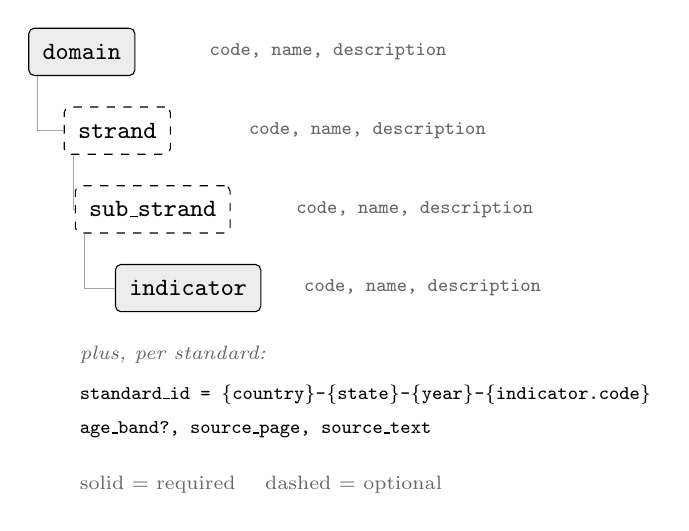
\begin{tikzpicture}[
  font=\small,
  lvl/.style={draw, rounded corners=2pt, minimum height=6mm, inner xsep=5pt, align=left},
  req/.style={lvl, fill=black!7},
  opt/.style={lvl, dashed, fill=white},
  ann/.style={font=\scriptsize\ttfamily, anchor=west, text=black!60},
  link/.style={-, gray!70}
]
\node[req] (d)  at (0,0)      {\texttt{domain}};
\node[opt] (s)  at (0.45,-1)  {\texttt{strand}};
\node[opt] (ss) at (0.90,-2)  {\texttt{sub\_strand}};
\node[req] (i)  at (1.35,-3)  {\texttt{indicator}};

\draw[link] (d.south west) ++(0.12,0) |- (s.west);
\draw[link] (s.south west) ++(0.12,0) |- (ss.west);
\draw[link] (ss.south west) ++(0.12,0) |- (i.west);

\node[ann] at (1.5,0)    {code, name, description};
\node[ann] at (2.0,-1)   {code, name, description};
\node[ann] at (2.6,-2)   {code, name, description};
\node[ann] at (2.7,-3)   {code, name, description};

\node[font=\scriptsize, anchor=west, text=black!60] at (-0.15,-3.85)
  {\textit{plus, per standard:}};
\node[font=\scriptsize\ttfamily, anchor=west] at (-0.15,-4.35)
  {standard\_id = \{country\}-\{state\}-\{year\}-\{indicator.code\}};
\node[font=\scriptsize\ttfamily, anchor=west] at (-0.15,-4.8)
  {age\_band?, source\_page, source\_text};

\node[font=\scriptsize, anchor=west, text=black!60] at (-0.15,-5.5)
  {solid = required \quad dashed = optional};
\end{tikzpicture}
\caption{The canonical schema. Four hierarchy levels, of which
\texttt{strand} and \texttt{sub\_strand} are optional; each carries a code, a
name and an optional description. A stored record is one indicator together
with its fully resolved ancestry, not a node in a tree (\S\ref{sec:schema}).}
\label{fig:schema}
\end{figure}


\section{Representative Golden Examples}
\label{sec:appendix-goldens}
% AUTO-GENERATED by paper/dai2027/make_tables.py -- do not hand-edit.
% Every field is copied from the golden files on disk.

The detector golden is a flat list of elements and the parser golden a nested record per standard. The two examples below show the conventions \S\ref{sec:method-parsing} turns on; descriptions are omitted, and codes and identifiers are reproduced in full.
\medskip

{\raggedright\noindent\textbf{KY detector golden: a \texttt{<Label> <id>} heading, whose label-and-id is the code}\par}
\smallskip
{\scriptsize\noindent
\begin{tabular}{@{}p{0.22\linewidth}p{0.72\linewidth}@{}}
\toprule
\texttt{level} & \texttt{sub\_\allowbreak{}strand} \\
\texttt{code} & \texttt{Benchmark 1.\allowbreak{}1} \\
\texttt{title} & Maintains focus and sustains attention. \\
\bottomrule
\end{tabular}\par}
\medskip

{\raggedright\noindent\textbf{KY parser golden: the same element, its label form resolved to a domain-qualified code}\par}
\smallskip
{\scriptsize\noindent
\begin{tabular}{@{}p{0.3\linewidth}p{0.64\linewidth}@{}}
\toprule
\texttt{standard\_id} & \texttt{US-\allowbreak{}KY-\allowbreak{}2021-\allowbreak{}AL.\allowbreak{}1.\allowbreak{}1.\allowbreak{}EASPT} \\
\texttt{domain.code} & \texttt{AL} \\
\texttt{domain.name} & Approaches to Learning \\
\texttt{strand.code} & \texttt{AL.\allowbreak{}1} \\
\texttt{strand.name} & Sustains attention and persists with challenging activities and experiences. \\
\texttt{sub\_strand.code} & \texttt{AL.\allowbreak{}1.\allowbreak{}1} \\
\texttt{sub\_strand.name} & Maintains focus and sustains attention. \\
\texttt{indicator.code} & \texttt{AL.\allowbreak{}1.\allowbreak{}1.\allowbreak{}EASPT} \\
\texttt{indicator.name} & Engages in an activity for a sustained period of time. \\
\bottomrule
\end{tabular}\par}
\medskip

{\raggedright\noindent\textbf{NV parser golden: a printed namespace that skips a level, so the sub-strand code does not extend the strand's}\par}
\smallskip
{\scriptsize\noindent
\begin{tabular}{@{}p{0.3\linewidth}p{0.64\linewidth}@{}}
\toprule
\texttt{standard\_id} & \texttt{US-\allowbreak{}NV-\allowbreak{}2023-\allowbreak{}SS.\allowbreak{}ID.\allowbreak{}PK1} \\
\texttt{domain.code} & \texttt{SS} \\
\texttt{domain.name} & Social Studies \\
\texttt{strand.code} & \texttt{SS.\allowbreak{}1} \\
\texttt{strand.name} & Demonstrate a basic awareness of self as an individual, within the context of a group and community. \\
\texttt{sub\_strand.code} & \texttt{SS.\allowbreak{}ID} \\
\texttt{sub\_strand.name} & Individual Development and Cultural Identity \\
\texttt{indicator.code} & \texttt{SS.\allowbreak{}ID.\allowbreak{}PK1} \\
\texttt{indicator.name} & Identify and describe characteristics of self that are unique from others. \\
\bottomrule
\end{tabular}\par}
\medskip


\section{Confidence Score Distribution}
\label{sec:appendix-confidence}

Table~\ref{tab:confidence-distribution} gives the detector's confidence
distribution by hierarchy level and by audit verdict, supporting
\S\ref{sec:lessons}. The score also drifts between runs: on an earlier freeze
of the same corpus, 89.7\% of indicators scored 0.95 or above, against 93.5\%
in the recorded run. The single confirmed hallucination is the lowest-scoring
element (0.90), but with one invented element in the corpus no threshold's
false-negative rate is measurable.

% AUTO-GENERATED by paper/dai2027/make_tables.py -- do not hand-edit.
% Source: paper/results/task8_20260904/confidence_distribution.json
% Regenerate with: python paper/dai2027/make_tables.py
\begin{table}[t]
  \centering
  \small
  \begin{tabular}{lrrr}
    \toprule
    & $n$ & \textbf{Range} & $\mathbf{\geq 0.95}$ \\
    \midrule
    \multicolumn{4}{l}{\emph{By hierarchy level}} \\
    domain & 16 & 0.95--0.97 & 16/16 \\
    strand & 51 & 0.92--0.97 & 48/51 \\
    sub-strand & 49 & 0.92--0.97 & 47/49 \\
    indicator & 263 & 0.90--0.97 & 246/263 \\
    \midrule
    \multicolumn{4}{l}{\emph{By audit verdict (in-scope only)}} \\
    matched a golden & 135 & 0.92--0.97 & 117/135 \\
    real, unannotated & 117 & 0.92--0.97 & 115/117 \\
    real, split title & 39 & 0.95--0.96 & 39/39 \\
    real, reprinted & 5 & 0.95 & 5/5 \\
    \textbf{invented} & 1 & 0.90 & 0/1 \\
    \midrule
    All & 379 & 0.90--0.97 & 357/379 \\
    \bottomrule
  \end{tabular}
  \caption{Detector self-reported confidence over the 379 elements of the recorded run (subset tier). The verdict rows cover the 297 detections inside the domains a golden annotates; the other 82 were not audited. The prompt asks for $\geq 0.95$ when the depth map clearly applies, $0.80$--$0.94$ when the chunk is ambiguous, and $<0.70$ when guessing; the score takes 5 distinct values in $[0.90, 0.97]$ and uses the bottom band never. \textbf{Nothing in the pipeline thresholds this score} (\S\ref{sec:lessons}).}
  \label{tab:confidence-distribution}
\end{table}


\section{Corpus}
\label{sec:appendix-corpus}

Table~\ref{tab:corpus-appendix} identifies every source document, and
Table~\ref{tab:corpus-pages} the pages each tier retains, so either tier can be
reconstructed from the issuing agency's copy.

% AUTO-GENERATED by paper/dai2027/make_tables.py (via generate_tables.build_corpus_appendix_table) -- do not hand-edit.
% Source: standards/standards_tracking.md, paper/results/corpus_tiers.json
% Regenerate with: python paper/analysis/generate_tables.py
% Corpus tier (guardrail 1): every row is the _only_subset tier, never full-document.
\begin{table*}[t]
\centering
\small
\begin{tabular}{llrlrrr}
\toprule
\textbf{State} & \textbf{Role} & \textbf{Year} & \textbf{Publisher} & \textbf{Full} & \textbf{Trim.} & \textbf{Subset} \\
\midrule
CA & dev & 2021 & CA Dept.\ of Education & 68 & -- & 13 \\
AZ & dev & 2018 & AZ Dept.\ of Education & 217 & 65 & 15 \\
TX & dev & 2022 & TX Education Agency & 87 & 71 & 9 \\
CO & dev & 2020 & CO Dept.\ of Early Childhood & 41 & 41 & 10 \\
NV & validation & 2023 & NV Dept.\ of Education & 98 & 71 & 15 \\
KY & validation & 2021 & Governor's Office of Early Childhood & 120 & 52 & 8 \\
\bottomrule
\end{tabular}
\caption{Corpus provenance. \emph{Full} is the published PDF; \emph{Trim.}\ removes non-standards matter while retaining every standard; \emph{Subset} is the one-to-two-domain excerpt the headline quality measurements use, and is a genuine reduction in coverage. Colorado's \emph{Full} is its 41-page Ages~3--5 publication. These are third-party state-agency documents, identified here rather than redistributed (see the Ethical Statement).}
\label{tab:corpus-appendix}
\end{table*}

% AUTO-GENERATED by paper/dai2027/make_tables.py -- do not hand-edit.
% Source: paper/results/corpus_page_ranges.json
% Regenerate with: python paper/dai2027/make_tables.py
\begin{table*}[t]
\centering
\small
\begin{tabular}{llrp{0.62\textwidth}}
\toprule
\textbf{State} & \textbf{Tier} & \textbf{pp} & \textbf{Retained PDF pages} \\
\midrule
AZ & trimmed & 65 & 2, 21, 23--28, 41, 43--50, 66, 70--82, 107, 110--120, 139, 142--145, 156, 158--162, 179, 181--185, 198, 201--204 (of 217) \\
AZ & subset & 15 & 2, 21, 23, 66, 70--78, 81--82 (of 217) \\
CA & subset & 13 & 1--5, 11--13, 18--22 (of 68) \\
CO & trimmed & 41 & 1--41 (of 41) \\
CO & subset & 10 & 1, 3--9, 11--12 (of 41) \\
TX & trimmed & 71 & 1, 9--65, 69--81 (of 87) \\
TX & subset & 9 & 1, 9--13, 59--61 (of 87) \\
NV & trimmed & 71 & 1, 3, 16--84 (of 98) \\
NV & subset & 15 & 1, 3, 23--26, 54--57, 61--65 (of 98) \\
KY & trimmed & 52 & 1, 52--102 (of 120) \\
KY & subset & 8 & 1, 52--55, 65, 71--72 (of 120) \\
\bottomrule
\end{tabular}
\caption{Pages each tier retains, as indices into the published PDF file. Printed page numbers differ by each document's front matter (Kentucky's PDF page 52 is printed page 39). Every tier page was matched by text to a published page. California has no trimmed tier.}
\label{tab:corpus-pages}
\end{table*}


\end{document}
